\documentclass{beamer}

\usepackage[ruled]{algorithm2e}
\SetKw{KwRet}{return}
\SetKwRepeat{Repeat}{repeat}{until}
\usepackage{amsmath}

\usetheme{AnnArbor}
\usecolortheme{crane}
\usefonttheme[onlymath]{serif}

\title{Deep Learning - Foundations and Concepts}
\subtitle{Chapter 20. Diffusion Models}
\author{nonlineark@github}
\date{\today}

\begin{document}

\begin{frame}
    \titlepage
\end{frame}

\begin{frame}
    \frametitle{Outline}
    \tableofcontents
\end{frame}

\section{Forward Encoder}

\begin{frame}
    \frametitle{Forward encoder}
    Suppose we take an image from the training set, which we will denote by $x$, and blend it with Gaussian noise independently for each pixel to give a noise-corrupted image $z_{1}$ defined by:
    \begin{align*}
        z_{1}&=\sqrt{1-\beta_{1}}x+\sqrt{\beta_{1}}\epsilon_{1}\qquad\epsilon_{1}\sim\mathcal{N}(\epsilon_{1};0,I) \\
        q(z_{1}|x)&=\mathcal{N}(z_{1};\sqrt{1-\beta_{1}}x,\beta_{1}I)
    \end{align*}
    where $\beta_{1}<1$ is the variance of the noise distribution.
\end{frame}

\begin{frame}
    \frametitle{Forward encoder}
    We then repeat the process with additional independent Gaussian noise steps to give a sequence of increasingly noisy images $z_{1},\hdots,z_{T}$:
    \begin{align*}
        z_{t}&=\sqrt{1-\beta_{t}}z_{t-1}+\sqrt{\beta_{t}}\epsilon_{t}\qquad\epsilon_{t}\sim\mathcal{N}(\epsilon_{t};0,I) \\
        q(z_{t}|z_{t-1})&=\mathcal{N}(z_{t};\sqrt{1-\beta_{t}}z_{t-1},\beta_{t}I)
    \end{align*}
    The values of the variance parameters $\beta_{t}\in(0,1)$ are set by hand and are typically chosen such that the variance values increase through the chain according to a prescribed schedule such that $\beta_{1}<\cdots<\beta_{T}$.
\end{frame}

\begin{frame}
    \frametitle{Diffusion kernel}
    Using induction, it's straightforward to verify that:
    \begin{align*}
        z_{t}&=\sqrt{\alpha_{t}}x+\sqrt{1-\alpha_{t}}\epsilon_{t}\qquad\epsilon_{t}\sim\mathcal{N}(\epsilon_{t};0,I) \\
        q(z_{t}|x)&=\mathcal{N}(z_{t};\sqrt{\alpha_{t}}x,(1-\alpha_{t})I)
    \end{align*}
    where we have defined:
    \begin{equation*}
        \alpha_{t}=\prod_{\tau=1}^{t}(1-\beta_{\tau})
    \end{equation*}
    We call $q(z_{t}|x)$ the diffusion kernel. After many steps the image becomes indistinguishable from Gaussian noise, and in the limit $T\to\infty$ we have:
    \begin{equation*}
        q(z_{T}|x)=\mathcal{N}(z_{T};0,I)
    \end{equation*}
\end{frame}

\begin{frame}
    \frametitle{Conditional distribution}
    Our goal is to learn to undo the noise process, and so it is natural to consider the reverse of the conditional distribution $q(z_{t}|z_{t-1})$:
    \begin{equation*}
        q(z_{t-1}|z_{t})=\frac{q(z_{t}|z_{t-1})q(z_{t-1})}{q(z_{t})}
    \end{equation*}
    But $q(z_{t-1})$ is difficult to calculate:
    \begin{itemize}
        \item Evaluation of the integral $\int{}q(z_{t-1}|x)p(x)\mathrm{d}x$ is intractable, because we must integrate over the unknown data density $p(x)$.
        \item If we approximate the integration using samples from the training data set, we obtain a complicated distribution expressed as a mixture of Gaussians.
    \end{itemize}
\end{frame}

\begin{frame}
    \frametitle{Conditional distribution}
    Instead, we consider the conditional version of the reverse distribution, conditioned on the data vector $x$, defined by $q(z_{t-1}|z_{t},x)$:
    \begin{align*}
        q(z_{t-1}|z_{t},x)&=\frac{q(z_{t}|z_{t-1},x)q(z_{t-1}|x)}{q(z_{t}|x)}=\frac{q(z_{t}|z_{t-1})q(z_{t-1}|x)}{q(z_{t}|x)} \\
        &=\mathcal{N}(z_{t-1};m_{t}(x,z_{t}),\sigma^{2}_{t}I) \\
        m_{t}(x,z_{t})&=\frac{(1-\alpha_{t-1})\sqrt{1-\beta_{t}}z_{t}+\sqrt{\alpha_{t-1}}\beta_{t}x}{1-\alpha_{t}} \\
        \sigma^{2}_{t}&=\frac{\beta_{t}(1-\alpha_{t-1})}{1-\alpha_{t}}
    \end{align*}
\end{frame}

\section{Reverse Decoder}

\begin{frame}
    \frametitle{Reverse decoder}
    \begin{itemize}
        \item The forward encoder model is defined by a sequence of Gaussian conditional distribution $q(z_{t}|z_{t-1})$ but inverting this directly leads to a distribution $q(z_{t-1}|z_{t})$ that is intractable.
        \item Instead, we will learn an approximation to the reverse distribution by using a distribution $p(z_{t-1}|z_{t};w)$ governed by a deep neural network, where $w$ represents the network weights and biases.
    \end{itemize}
    \begin{figure}
        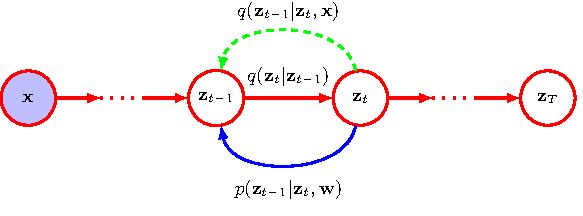
\includegraphics{Figure_2.pdf}
    \end{figure}
\end{frame}

\begin{frame}
    \frametitle{Reverse decoder}
    For $\beta_{t}\ll{}1$, the distribution $q(z_{t-1}|z_{t})$ will be approximately a Gaussian distribution over $z_{t-1}$ (\href{https://arxiv.org/pdf/1503.03585}{further references}). We therefore model the reverse process using a Gaussian distribution of the form:
    \begin{equation*}
        p(z_{t-1}|z_{t};w)=\mathcal{N}(z_{t-1};\mu(z_{t},t;w),\beta_{t}I)
    \end{equation*}
    where $\mu(z_{t},t;w)$ is a deep neural network governed by a set of parameters $w$. Note:
    \begin{itemize}
        \item The network takes the step index $t$ explicitly as an input so that it can account for the variation of the variance $\beta_{t}$ across different steps of the chain.
        \item It is also possible to learn the covariances of the denoising process by incorporating further outputs in the network to account for the curvature in the distribution $q(z_{t-1})$ in the neighborhood of $z_{t}$.
    \end{itemize}
\end{frame}

\begin{frame}
    \frametitle{Reverse decoder}
    The overall reverse denoising process then takes the form of a Markov chain given by:
    \begin{align*}
        p(x,z_{1},\hdots,z_{T};w)&=p(z_{T})\prod_{t=2}^{T}p(z_{t-1}|z_{t};w)p(x|z_{1};w) \\
        p(z_{T})&=q(z_{T})=\mathcal{N}(z_{T};0,I)
    \end{align*}
    Once the model has been trained, sampling is straightforward, we just follow the chain $z_{T},\hdots,z_{1},x$ in turn.
\end{frame}

\begin{frame}
    \frametitle{Training the decoder}
    The likelihood function is given by:
    \begin{equation*}
        p(x;w)=\int{}p(x,z_{1},\hdots,z_{T};w)\mathrm{d}z_{1}\cdots\mathrm{d}z_{T}
    \end{equation*}
    We see that the likelihood involves integrating over all possible trajectories by which noise samples could give rise to the observed data point. The integrals are intractable.
\end{frame}

\begin{frame}
    \frametitle{Evidence lower bound}
    \begin{itemize}
        \item Since the exact likelihood is intractable, we can adopt a similar approach to that used with variational autoencoders and maximize the evidence lower bound.
        \item With diffusion models, we choose $q(z)$ to be given by the fixed distribution $q(z_{1},\hdots,z_{T}|x)$, and so the only adjustable parameters are those in the model $p(x,z_{1},\hdots,z_{T};w)$ for the reverse Markov chain.
    \end{itemize}
\end{frame}

\begin{frame}
    \frametitle{Evidence lower bound}
    \begin{align*}
        \mathcal{L}(w)&=\int{}q(z)\log\frac{p(x,z;w)}{q(z)}\mathrm{d}z \\
        &=E_{q}(\log\frac{p(z_{T})\prod_{t=2}^{T}p(z_{t-1}|z_{t};w)p(x|z_{1};w)}{q(z_{1}|x)\prod_{t=2}^{T}q(z_{t}|z_{t-1},x)}) \\
        &=E_{q}(\log{}p(z_{T})-\log{}q(z_{1}|x)+\log{}p(x|z_{1};w) \\
        &\qquad+\sum_{t=2}^{T}\log\frac{p(z_{t-1}|z_{t};w)}{q(z_{t}|z_{t-1},x)})
    \end{align*}
\end{frame}

\begin{frame}
    \frametitle{Evidence lower bound}
    \begin{itemize}
        \item The first and second terms are independent of $w$ and can be omitted.
        \item The third term can be evaluated by approximating the expectation by a Monte Carlo estimate: $E_{q}(\log{}p(x|z_{1};w))\approx\frac{1}{L}\sum_{l=1}^{L}\log{}p(x|z_{1}^{(l)};w)$, where $z_{1}^{(l)}\sim\mathcal{N}(z_{1};\sqrt{1-\beta_{1}}x,\beta_{1}I)$.
        \item For the fourth term:
        \begin{itemize}
            \item Although we can sample from $q(z_{t-1}|x)$ and $q(z_{t}|z_{t-1})$, the use of pairs of sampled values creates very noisy estimates with high variance, so that an unnecessarily large number of samples is required.
            \item Instead, we rewrite the ELBO in a form that can be estimated by sampling just one value per term.
        \end{itemize}
    \end{itemize}
\end{frame}

\begin{frame}
    \frametitle{Rewriting the ELBO}
    Following our discussion of the ELBO for the variational autoencoder, our goal here is to write the ELBO in terms of Kullback-Leibler divergences:
    \begin{align*}
        q(z_{t}|z_{t-1},x)&=\frac{q(z_{t-1}|z_{t},x)q(z_{t}|x)}{q(z_{t-1}|x)} \\
        \log\frac{p(z_{t-1}|z_{t};w)}{q(z_{t}|z_{t-1},x)}&=\log\frac{p(z_{t-1}|z_{t};w)}{q(z_{t-1}|z_{t},x)}+\log\frac{q(z_{t-1}|x)}{q(z_{t}|x)}
    \end{align*}
    The second term is independent of $w$ and can be omitted:
    \begin{align*}
        \mathcal{L}(w)&=E_{q}(\log{}p(x|z_{1};w))+\sum_{t=2}^{T}E_{q}(\log\frac{p(z_{t-1}|z_{t};w)}{q(z_{t-1}|z_{t},x)})
    \end{align*}
\end{frame}

\begin{frame}
    \frametitle{Rewriting the ELBO}
    \begin{align*}
        &E_{q}(\log{}p(x|z_{1};w))=\int{}q(z_{1}|x)p(x|z_{1};w)\mathrm{d}z_{1}=\textrm{reconstruction term} \\
        &E_{q}(\log\frac{p(z_{t-1}|z_{t};w)}{q(z_{t-1}|z_{t},x)}) \\
        &=\int\bigg(\int\bigg(\int{}q(z_{1}|x)\cdots{}q(z_{t-1}|z_{t-2})\mathrm{d}z_{1}\cdots\mathrm{d}z_{t-2}\bigg) \\
        &\qquad\frac{q(z_{t-1}|z_{t},x)}{q(z_{t-1}|x)}\log\frac{p(z_{t-1}|z_{t};w)}{q(z_{t-1}|z_{t},x)}\mathrm{d}z_{t-1}\bigg)q(z_{t}|x)\mathrm{d}z_{t} \\
        &=-\int\mathrm{KL}(q(z_{t-1}|z_{t},x)||p(z_{t-1}|z_{t};w))q(z_{t}|x)\mathrm{d}z_{t} \\
        &=\textrm{consistency term}
    \end{align*}
\end{frame}

\begin{frame}
    \frametitle{Rewriting the ELBO}
    The consistency terms are defined between pairs of Gaussian distributions and therefore can be expressed in closed form:
    \begin{align*}
        &\mathrm{KL}(q(z_{t-1}|z_{t},x)||p(z_{t-1}|z_{t};w))=\frac{1}{2\beta_{t}}||m_{t}(x,z_{t})-\mu(z_{t},t;w)||^{2}+\textrm{const} \\
        &-\int\mathrm{KL}(q(z_{t-1}|z_{t},x)||p(z_{t-1}|z_{t};w))q(z_{t}|x)\mathrm{d}z_{t} \\
        &=-\frac{1}{2\beta_{t}}\int||m_{t}(x,z_{t})-\mu(z_{t},t;w)||^{2}q(z_{t}|x)\mathrm{d}z_{t}+\textrm{const} \\
        &\approx-\frac{1}{2\beta_{t}}\frac{1}{L}\sum_{l=1}^{L}||m_{t}(x,z_{t}^{(l)})-\mu(z_{t}^{(l)},t;w)||^{2}+\textrm{const}
    \end{align*}
    where $z_{t}^{(l)}\sim\mathcal{N}(z_{t};\sqrt{\alpha_{t}}x,(1-\alpha_{t})I)$, and any additive terms that are independent of the network parameters $w$ have been absorbed into the constant term. 
\end{frame}

\begin{frame}
    \frametitle{Predicting the noise}
    Let's further simplify the training objective $\mathcal{L}(w)$ by changing the role of the neural network so that instead of predicting the denoised image at each step of the Markov chain it predicts the total noise component that was added to the original image to create the noisy image at that step:
    \begin{align*}
        z_{t}&=\sqrt{\alpha_{t}}x+\sqrt{1-\alpha_{t}}\epsilon_{t}\implies{}x=\frac{1}{\sqrt{\alpha_{t}}}z_{t}-\frac{\sqrt{1-\alpha_{t}}}{\sqrt{\alpha_{t}}}\epsilon_{t} \\
        m_{t}(x,z_{t})&=\frac{(1-\alpha_{t-1})\sqrt{1-\beta_{t}}z_{t}+\sqrt{\alpha_{t-1}}\beta_{t}x}{1-\alpha_{t}} \\
        &=\frac{1}{\sqrt{1-\beta_{t}}}(z_{t}-\frac{\beta_{t}}{\sqrt{1-\alpha_{t}}}\epsilon_{t})
    \end{align*}
\end{frame}

\begin{frame}
    \frametitle{Predicting the noise}
    We introduce a neural network $g(z_{t},t;w)$ that aims to predict the total noise that was added to $x$ to generate $z_{t}$:
    \begin{equation*}
        \mu(z_{t},t;w)=\frac{1}{\sqrt{1-\beta_{t}}}(z_{t}-\frac{\beta_{t}}{\sqrt{1-\alpha_{t}}}g(z_{t},t;w))
    \end{equation*}
    We see that:
    \begin{align*}
        \mathrm{KL}&(q(z_{t-1}|z_{t},x)||p(z_{t-1}|z_{t};w))=\frac{1}{2\beta_{t}}||m_{t}(x,z_{t})-\mu(z_{t},t;w)||^{2}+\textrm{const} \\
        &=\frac{\beta_{t}}{2(1-\alpha_{t})(1-\beta_{t})}||g(z_{t},t;w)-\epsilon_{t}||^{2}+\textrm{const}
    \end{align*}
\end{frame}

\begin{frame}
    \frametitle{Predicting the noise}
    Furthermore, for the reconstruction term, we have:
    \begin{align*}
        \log{}p(x|z_{1};w)&=-\frac{1}{2\beta_{1}}||x-\mu(z_{1},1;w)||^{2}+\textrm{const} \\
        &=-\frac{1}{2(1-\beta_{1})}||g(z_{1},1;w)-\epsilon_{1}||^{2}+\textrm{const}
    \end{align*}
    Now the reconstruction and consistency terms can be combined:
    \begin{equation*}
        \mathcal{L}(w)=-\sum_{t=1}^{T}\frac{\beta_{t}}{2(1-\alpha_{t})(1-\beta_{t})}\int||g(z_{t},t;w)-\epsilon_{t}||^{2}q(z_{t}|x)\mathrm{d}z_{t}
    \end{equation*}
\end{frame}

\begin{frame}
    \frametitle{Predicting the noise}
    It is found empirically that performance is further improved simply by omitting the factor $\frac{\beta_{t}}{2(1-\alpha_{t})(1-\beta_{t})}$, so that all steps in the Markov chain have equal weighting. If we only do one sample for each $\epsilon_{t}$, then we have:
    \begin{equation*}
        \mathcal{L}(w)=-\sum_{t=1}^{T}||g(\sqrt{\alpha_{t}}x+\sqrt{1-\alpha_{t}}\epsilon_{t},t;w)-\epsilon_{t}||^{2}
    \end{equation*}
\end{frame}

\begin{frame}
    \frametitle{Predicting the noise}
    \begin{algorithm}[H]
        \caption{Training a denoising diffusion probabilistic model}
        \For{$t\gets{}1$ \KwTo $T$}{
            $\alpha_{t}\gets\prod_{\tau=1}^{t}(1-\beta_{\tau})$\;
        }
        \Repeat{converged}{
            $x\sim\mathcal{D}$\;
            $t\sim\{1,\hdots,T\}$\;
            $\epsilon\sim\mathcal{N}(\epsilon;0,I)$\;
            $z_{t}\gets\sqrt{\alpha_{t}}x+\sqrt{1-\alpha_{t}}\epsilon$\;
            $\mathcal{L}(w)\gets||g(z_{t},t;w)-\epsilon||^{2}$\;
            Take optimizer step
        }
        \Return{$w$}\;
    \end{algorithm}
\end{frame}

\begin{frame}
    \frametitle{Generating new samples}
    \begin{algorithm}[H]
        \caption{Sampling from a denoising diffusion probabilistic model}
        $z_{T}\sim\mathcal{N}(z_{T};0,I)$\;
        \For{$t\gets{}T$ \KwTo $2$}{
            $\alpha_{t}\gets\prod_{\tau=1}^{t}(1-\beta_{\tau})$\;
            $\mu(z_{t},t;w)\gets\frac{1}{\sqrt{1-\beta_{t}}}(z_{t}-\frac{\beta_{t}}{\sqrt{1-\alpha_{t}}}g(z_{t},t;w))$\;
            $\epsilon\sim\mathcal{N}(\epsilon;0,I)$\;
            $z_{t-1}\gets\mu(z_{t},t;w)+\sqrt{\beta_{t}}\epsilon$\;
        }
        $x\gets\frac{1}{\sqrt{1-\beta_{1}}}(z_{1}-\frac{\beta_{1}}{\sqrt{1-\alpha_{1}}}g(z_{1},1;w))$\;
        \Return{$x$}\;
    \end{algorithm}
\end{frame}

\section{Score Matching}

\begin{frame}
    \frametitle{Score function}
    Score function is defined as the gradient of the log likelihood with respect to the data vector $x$ and is given by:
    \begin{equation*}
        s(x)=\nabla_{x}\log{}p(x)
    \end{equation*}
    \begin{figure}
        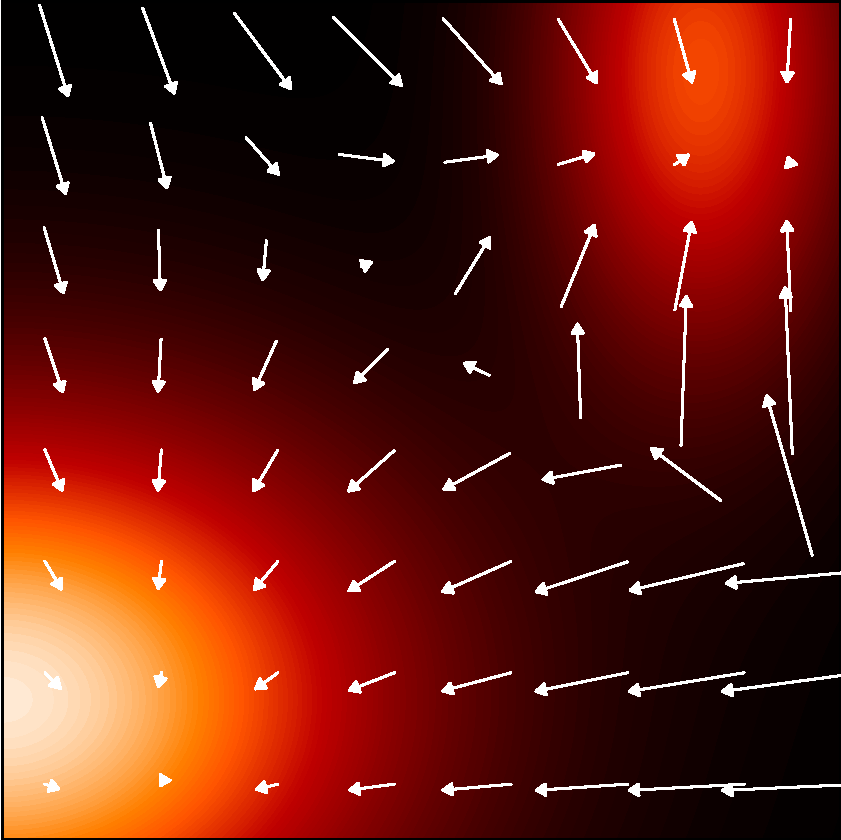
\includegraphics[height=0.5\textheight]{Figure_5.pdf}
    \end{figure}
\end{frame}

\begin{frame}
    \frametitle{Score loss function}
    To train such a model we need to define a loss function that aims to match the model score function $s(x;w)$ to the score function $\nabla_{x}\log{}p(x)$ of the distribution $p(x)$ that generated the data. An example:
    \begin{equation*}
        J(w)=\frac{1}{2}\int||s(x;w)-\nabla_{x}\log{}p(x)||^{2}p(x)\mathrm{d}x
    \end{equation*}
\end{frame}

\begin{frame}
    \frametitle{Score loss function}
    There are broadly two ways to represent the score function $s(x;w)$ using a deep neural network:
    \begin{itemize}
        \item Because $\nabla_{x}\log{}p(x)=\frac{\nabla_{x}p(x)}{p(x)}$ has the same dimensionality as $x$, the first approach is to have a network with the same number of outputs as inputs.
        \begin{itemize}
            \item The learned function may not be a gradient of a scalar function.
        \end{itemize}
        \item An alternative approach is to have a network with a single output $\phi(x)$ and then to compute $\nabla_{x}\phi(x)$ using automatic differentiation.
        \begin{itemize}
            \item This second approach is computationally more expensive.
        \end{itemize}
    \end{itemize}
\end{frame}

\begin{frame}
    \frametitle{Modified score loss}
    We do not know the true data distribution $p(x)$. All we have is the finite data set $\mathcal{D}=\{x_{1},\hdots,x_{N}\}$ from which we can construct an empirical distribution:
    \begin{equation*}
        p_{\mathcal{D}}(x)=\frac{1}{N}\sum_{n=1}^{N}\delta(x-x_{n})
    \end{equation*}
    where $\delta$ is the Dirac delta function. Now $p_{\mathcal{D}}$ is not a differentiable function of $x$, we need to introduce a noise model to smear out the data points:
    \begin{equation*}
        q_{\sigma}(z)=\int{}q_{\sigma}(z|x)p(x)\mathrm{d}x
    \end{equation*}
    where $q_{\sigma}(z|x)$ is the noise kernel, and $q_{\sigma}(z)$ is known as a Parzen estimator.
\end{frame}

\begin{frame}
    \frametitle{Modified score loss}
    We can now use the corresponding loss with respect to the smoothed Parzen density in the form:
    \begin{align*}
        &J(w)=\frac{1}{2}\int||s(z;w)-\nabla_{z}\log{}q_{\sigma}(z)||^{2}q_{\sigma}(z)\mathrm{d}z \\
        &=\frac{1}{2}\int(||s(z;w)||^{2}q_{\sigma}(z)-2(s(z;w)\cdot\nabla_{z}q_{\sigma}(z)))\mathrm{d}z+C \\
        &=\frac{1}{2}\int\bigg(\int||s(z;w)||^{2}q_{\sigma}(z|x)p(x)\mathrm{d}x \\
        &\qquad-\int{}2(s(z;w)\cdot\nabla_{z}q_{\sigma}(z|x))p(x)\mathrm{d}x\bigg)\mathrm{d}z+C \\
        &=\frac{1}{2}\iint(||s(z;w)||^{2}-2(s(z;w)\cdot\nabla_{z}\log{}q_{\sigma}(z|x)))q_{\sigma}(z|x)p(x)\mathrm{d}x\mathrm{d}z+C \\
        &=\frac{1}{2}\iint||s(z;w)-\nabla_{z}\log{}q_{\sigma}(z|x)||^{2}q_{\sigma}(z|x)p(x)\mathrm{d}x\mathrm{d}z+C
    \end{align*}
\end{frame}

\begin{frame}
    \frametitle{Modified score loss}
    If we substitute for $p(x)$ using the empirical density $p_{\mathcal{D}}(x)$, we obtain:
    \begin{equation*}
        J(w)=\frac{1}{2N}\sum_{n=1}^{N}\int||s(z;w)-\nabla_{z}\log{}q_{\sigma}(z|x_{n})||^{2}q_{\sigma}(z|x_{n})\mathrm{d}z+C
    \end{equation*}
\end{frame}

\begin{frame}
    \frametitle{Modified score loss}
    For the Gaussian Parzen kernel $q_{\sigma}(z|x)=\mathcal{N}(z;x,\sigma^{2}I)$, the score function becomes:
    \begin{equation*}
        \nabla_{z}\log{}q_{\sigma}(z|x)=-\frac{z-x}{\sigma^{2}}=-\frac{1}{\sigma}\epsilon\qquad\epsilon\sim\mathcal{N}(\epsilon;0,I)
    \end{equation*}
    If we consider the specific noise model $q(z|x)=\mathcal{N}(z;\sqrt{\alpha_{t}}x,(1-\alpha_{t})I)$ then we obtain:
    \begin{equation*}
        \nabla_{z}\log{}q(z|x)=-\frac{1}{\sqrt{1-\alpha_{t}}}\epsilon\qquad\epsilon\sim\mathcal{N}(\epsilon;0,I)
    \end{equation*}
    We see that the score loss measures the difference between the neural network prediction and the noise $\epsilon$, and denoising score matching has close connection to denoising diffusion models.
\end{frame}

\begin{frame}
    \frametitle{Modified score loss}
    Having trained a score-based model, we can use Langevin dynamics to draw new samples:
    \begin{equation*}
        z^{(\tau+1)}=z^{(\tau)}+\eta{}s(z^{(\tau)};w)+\sqrt{2\eta}\epsilon^{(\tau)}\qquad\epsilon^{(\tau)}\sim\mathcal{N}(\epsilon;0,I)
    \end{equation*}
    \begin{figure}
        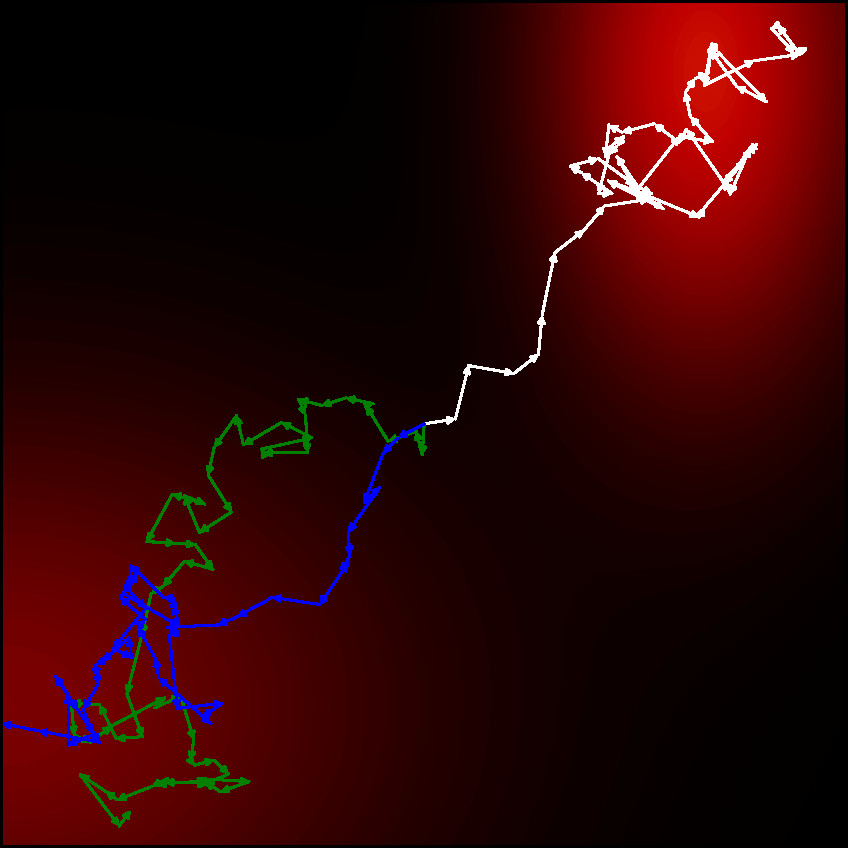
\includegraphics[height=0.5\textheight]{Figure_6.pdf}
    \end{figure}
\end{frame}

\end{document}